% PolitiKAST generated figure snippets.
% Use PDF for paper builds; PNG/SVG variants are available for slides.
% Numeric result figures must keep their caution text in the caption unless
% the underlying artifact is replaced by calibrated experiment output.

\begin{figure}[t]
\centering
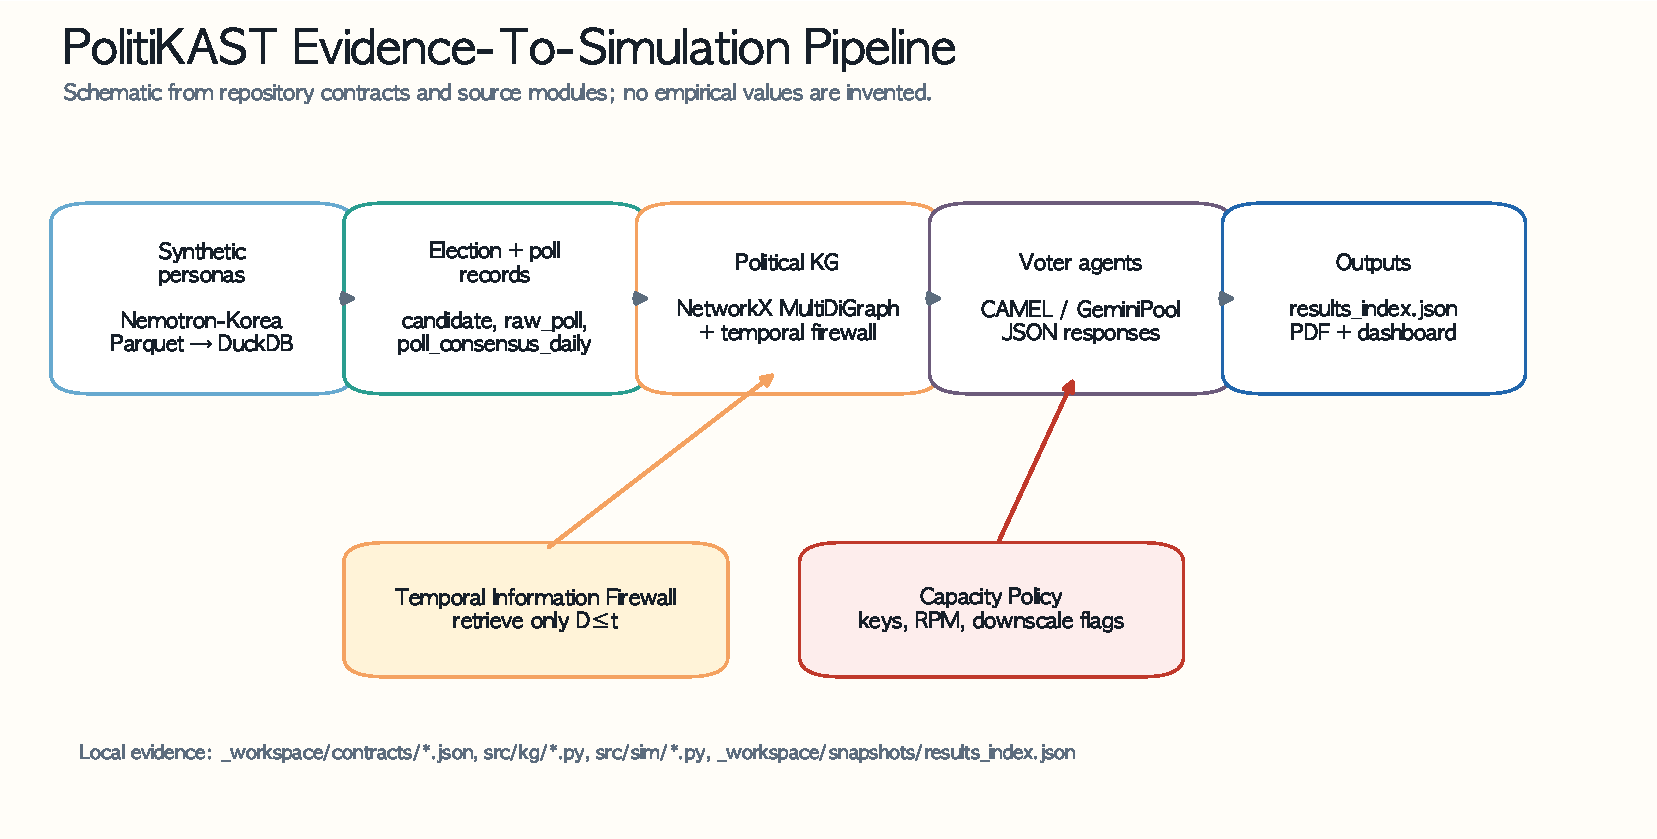
\includegraphics[width=\linewidth]{assets/fig_pipeline_architecture.pdf}
\caption{PolitiKAST end-to-end pipeline: persona substrate, election and poll records, political KG, LLM voter agents, and output artifacts. This is a schematic derived from repository contracts and source modules, not an empirical result figure.}
\label{fig:pipeline-architecture}
\end{figure}

\begin{figure}[t]
\centering
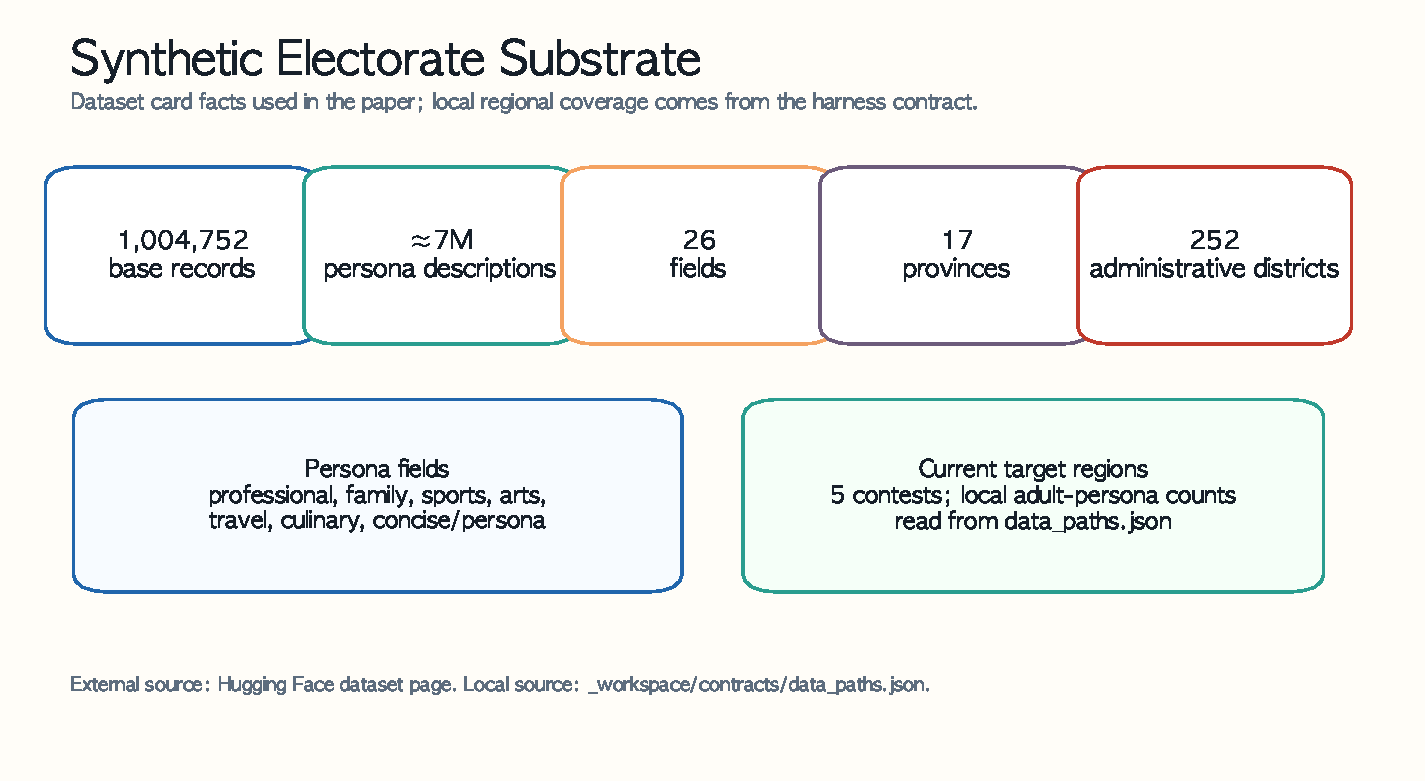
\includegraphics[width=\linewidth]{assets/fig_persona_data_card.pdf}
\caption{Data card for the synthetic Korean electorate substrate used by PolitiKAST. Dataset-level facts are externally sourced; regional coverage values are local harness contract values and should not be interpreted as official electorate sizes.}
\label{fig:persona-data-card}
\end{figure}

\begin{figure}[t]
\centering
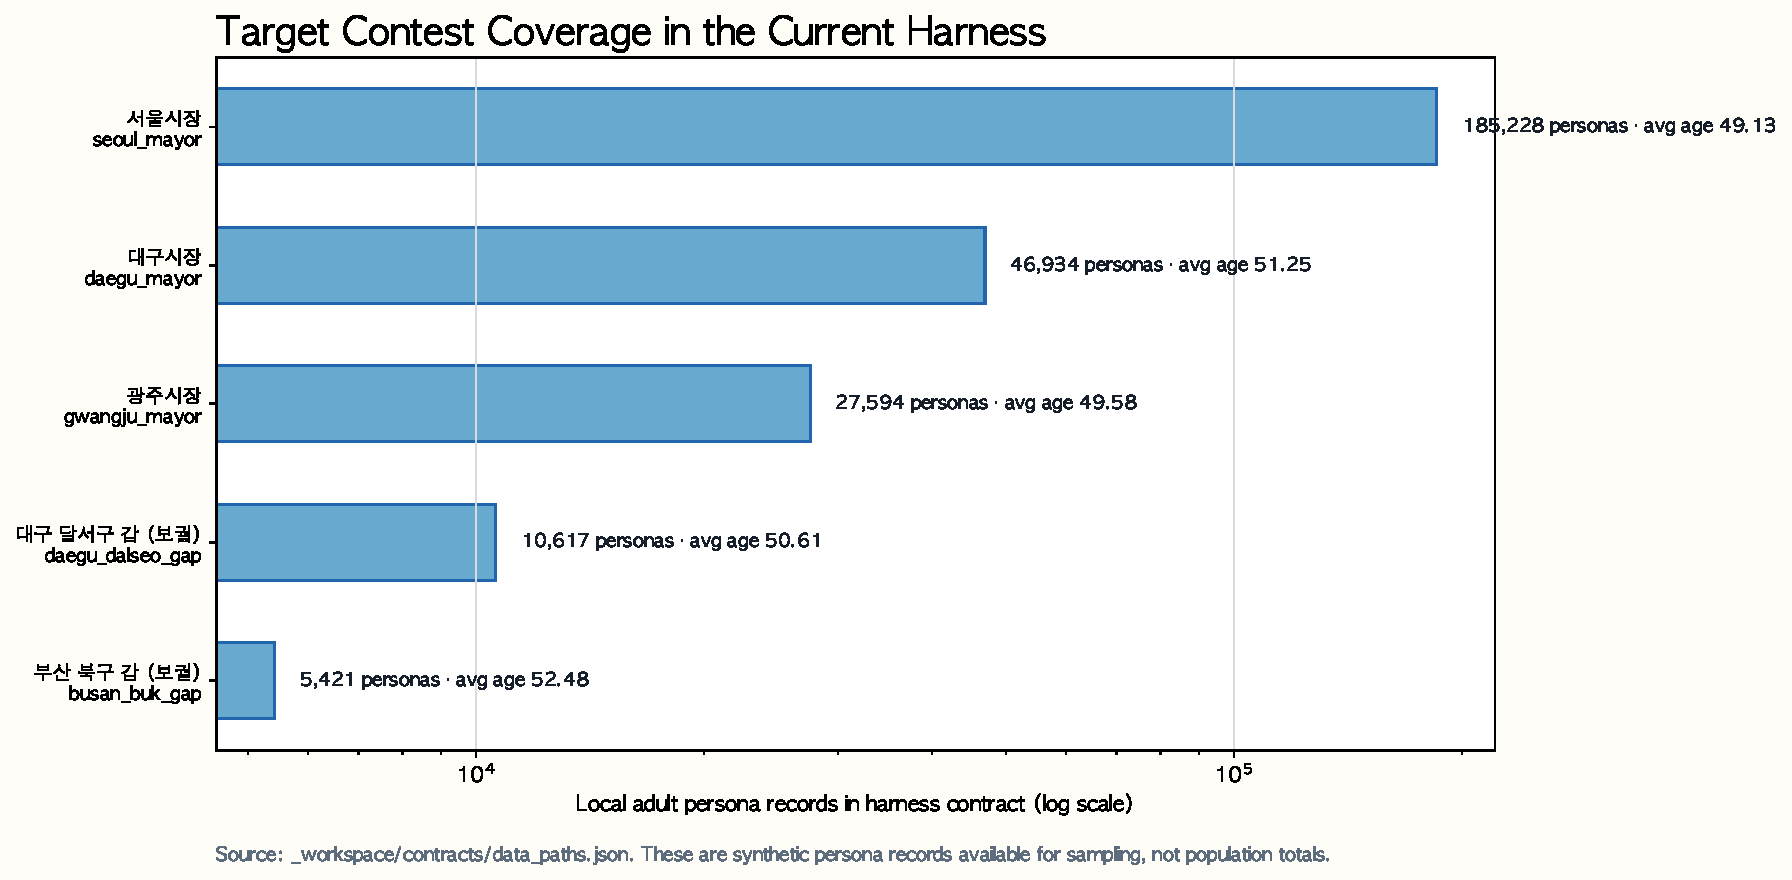
\includegraphics[width=\linewidth]{assets/fig_target_region_coverage.pdf}
\caption{Synthetic adult-persona coverage for the five target contests in the current harness. Counts come from \texttt{\_workspace/contracts/data\_paths.json}.}
\label{fig:target-region-coverage}
\end{figure}

\begin{figure}[t]
\centering
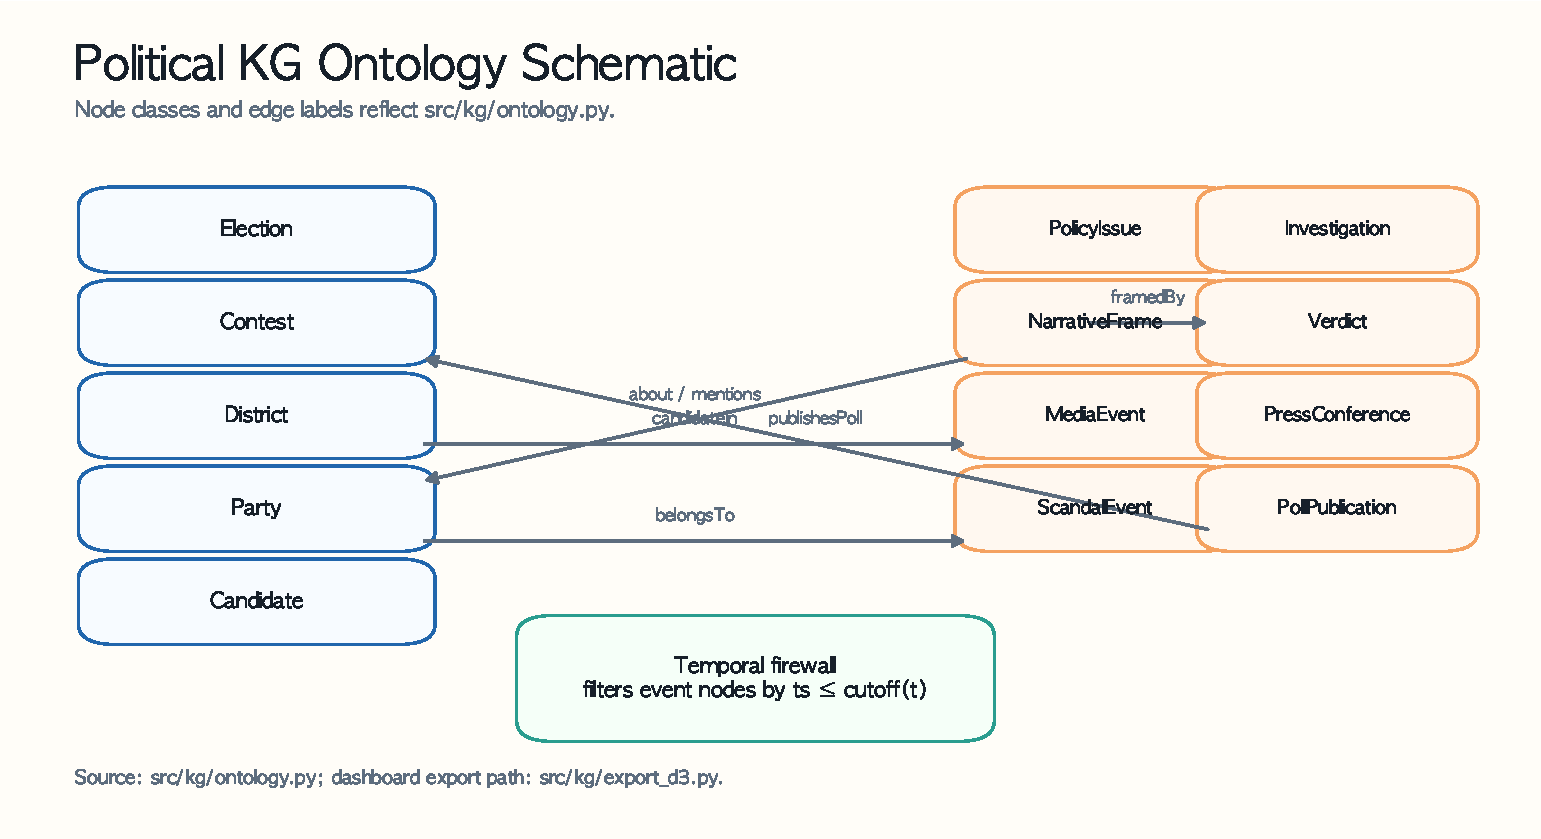
\includegraphics[width=\linewidth]{assets/fig_kg_ontology_schematic.pdf}
\caption{Schematic of PolitiKAST's election and discourse KG ontology, derived from \texttt{src/kg/ontology.py}.}
\label{fig:kg-ontology-schematic}
\end{figure}

\begin{figure}[t]
\centering
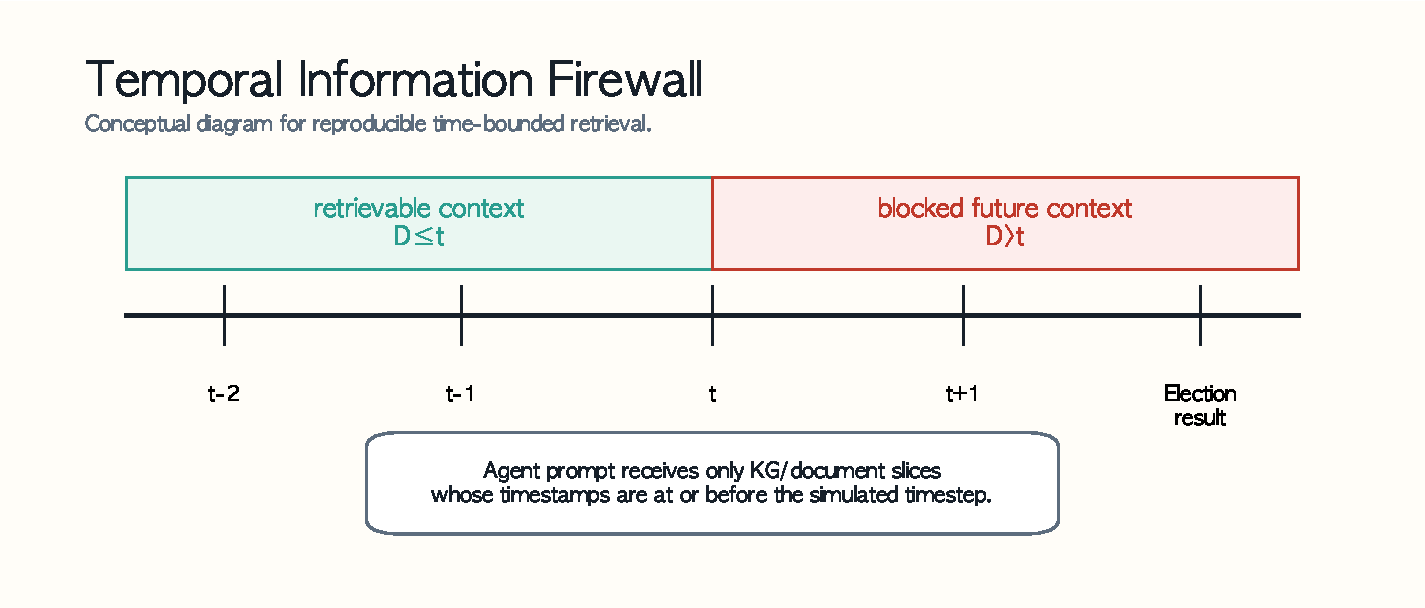
\includegraphics[width=\linewidth]{assets/fig_temporal_firewall.pdf}
\caption{Temporal information firewall used to prevent future information from entering voter-agent prompts.}
\label{fig:temporal-firewall}
\end{figure}
